% SPDX-License-Identifier: CC-BY-4.0
% Copyright (c) 2026 Alexander Stephen Donahue
\documentclass[11pt,reqno]{amsart}

\usepackage[T1]{fontenc}
\usepackage[utf8]{inputenc}
\usepackage{lmodern}
\usepackage{microtype}
\usepackage{amsmath,amssymb,amsthm,mathtools}
\usepackage{booktabs}
\usepackage{array}
\usepackage{tabularx}
\usepackage{longtable}
\usepackage{graphicx}
\usepackage{xcolor}
\usepackage{enumitem}
\usepackage[margin=1.0in]{geometry}
\usepackage[colorlinks=true,linkcolor=oiBlue,citecolor=oiGreen,urlcolor=oiBlue]{hyperref}
\newcommand{\code}[1]{\texttt{\small\nolinkurl{#1}}}
\newcommand{\cmd}[1]{\texttt{\small #1}}
\raggedbottom

% Okabe-Ito publication colors
\definecolor{oiBlue}{HTML}{0072B2}
\definecolor{oiVerm}{HTML}{D55E00}
\definecolor{oiGreen}{HTML}{009E73}
\definecolor{oiDark}{HTML}{1F2937}
\definecolor{oiBg}{HTML}{F8FAFC}
\definecolor{oiRule}{HTML}{CBD5E1}

% Theorem environments
\theoremstyle{plain}
\newtheorem{theorem}{Theorem}[section]
\newtheorem{proposition}[theorem]{Proposition}
\newtheorem{lemma}[theorem]{Lemma}
\newtheorem{corollary}[theorem]{Corollary}

\theoremstyle{definition}
\newtheorem{definition}[theorem]{Definition}
\newtheorem{example}[theorem]{Example}

\theoremstyle{remark}
\newtheorem{remark}[theorem]{Remark}
\newtheorem{openproblem}[theorem]{Open Problem}

% Epistemic status badges (non-breaking)
\newcommand{\tagLean}{\mbox{\textsf{\textbf{\color{oiBlue}[LEAN-6K]}}}}
\newcommand{\tagComp}{\mbox{\textsf{\textbf{\color{oiGreen}[EXACT-COMP]}}}}
\newcommand{\tagOpen}{\mbox{\textsf{\textbf{\color{oiVerm}[OPEN]}}}}

% Mathematical macros
\newcommand{\CD}{\mathrm{CD}}
\newcommand{\R}{\mathbb{R}}
\newcommand{\C}{\mathbb{C}}
\newcommand{\HH}{\mathbb{H}}
\newcommand{\OO}{\mathbb{O}}
\newcommand{\SSed}{\mathbb{S}_{16}}
\newcommand{\Z}{\mathbb{Z}}
\newcommand{\Q}{\mathbb{Q}}
\newcommand{\F}{\mathbb{F}}
\newcommand{\N}{\mathbb{N}}
\newcommand{\std}{\mathrm{std}}
\newcommand{\comp}{\mathrm{comp}}
\newcommand{\pop}{\mathrm{popcount}}
\newcommand{\parbit}{\mathrm{parity}}
\newcommand{\flip}{\mathrm{flip}}
\newcommand{\Ann}{\mathrm{Ann}}
\DeclareMathOperator{\rk}{rank}

\title[Cayley--Dickson Terrace Law, Mirror Conservation \& Dim-64 Rupture]{%
  The Dyadic-Palindromic Terrace Law, Nilpotent Mirror Conservation,\\
  and the Dimension-64 Hurwitz--Radon Rupture Across\\
  Generalized Cayley--Dickson Algebras%
}

\author{Alexander Stephen Donahue}
\address{Independent Researcher, Spokane, WA, USA}
\email{0\_0@0thernes.art}
\thanks{ORCID: \href{https://orcid.org/0009-0006-8168-9648}{0009-0006-8168-9648}.
Repository, six-kernel Lean~4.35.0 proofs, Rust/C11/Python engines, and interactive WebGL observatory:
\url{https://github.com/0thernes/cayley-dickson-terrace-frontier}. Archive ID: \texttt{0TH-2026-017}.}

\subjclass[2020]{Primary 17A35, 17A75, 11E25; Secondary 05C69, 68V20}
\keywords{Cayley--Dickson algebras, sedenions, zero divisors, Hurwitz--Radon numbers,
sums-of-squares composition, Box-Kites, Lean~4 formal verification}

\begin{document}

\begin{abstract}
We establish four interconnected structural theorems governing zero-divisor nullity spectra,
signature deformations, and norm-multiplicative subspaces across the entire infinite tower of
generalized Cayley--Dickson algebras $\CD_n(\gamma)$ of dimension $2^n$ ($n \ge 1$,
$\gamma \in \{\pm 1\}^n$).

\emph{First (Nilpotent Mirror Conservation)}, we prove that the generalized basis sign cocycle
factorizes universally as
$\sigma_n^\gamma(i,j) = \sigma_n^{\std}(i,j)(-1)^{\pop(i\,\&\,j\,\&\,\flip(\gamma))}$,
forcing every $2\times 2$ left-multiplication block determinant $\delta_n^\gamma(i,j,k)$ of a
basis 2-blade $e_i + e_j$ to flip by a sign completely independent of the block index $k$.
Consequently, non-nilpotent 2-blades preserve their Euclidean nullity while nilpotent 2-blades
undergo exact mirror inversion $\nu_n^\gamma(i,j) = 2^{n-1} - \nu_n^{\std}(i,j)$, conserving
every mirror-pair histogram sum $H_n^\gamma(v) + H_n^\gamma(2^{n-1}-v)$ and pinning the
midpoint stratum $H_n^\gamma(2^{n-2})$ across all $2^n$ signatures.

\emph{Second (The Dyadic-Palindromic Terrace Law)}, we derive an exact four-branch doubling
recurrence for Euclidean 2-blade nullity, yielding closed-form all-$n$ laws for total nullity
mass $M_n = 8(2^{n-1}-1)(2^{n-2}-1)(2^{n-3}-1)$, zero-divisor-free counts
$H_n^{\std}(0) = (6n-9)2^{n-2}+3$, exact even/odd bin interleaving
$H_{n+1}^{\std}(8m) = H_{n+1}^{\std}(2^n-4-8m) = 2H_n^{\std}(4m)$, interior palindromic
symmetry, an exact top-bin jump $3(2^n-2)$, sharp separation from the Biss--Dugger--Isaksen
annihilator ceiling $2^n - 4n + 4$ for every $n \ge 5$ (with uniqueness of equality at $n=4$),
and the crowning \emph{Universal Midpoint 42 Law}: $H_n^\gamma(2^{n-2}) = 42 \cdot 2^{n-4}$
for all $n \ge 4$ and all $2^n$ signatures $\gamma$.

\emph{Third (The Dimension-64 Hurwitz--Radon Bott Rupture)}, we determine the exact doubling
law and clique number of the basis right-compatibility graph $G_n^{\comp}$, proving
$\omega(G_n^{\comp}) = n+5$ for every $n \ge 3$ and uniqueness of the two universal
right-multipliers $\{e_0, e_{2^{n-1}}\}$ for all $n \ge 4$. Thus Cayley--Dickson coordinate
multiplication saturates the Hurwitz--Radon ceiling $\rho(2^n)$ at dimensions $8, 16, 32$
($8, 9, 10$), but suffers an irrevocable Bott-periodicity rupture at dimension~$64$
($11 < 12 = \rho(64)$) with diverging deficit $\rho(2^n) - (n+5) \ge n-5$ for all $n \ge 6$,
while an explicit doubling tower realizes $[2^{n-1}, 2(n+4), 2^n]$ pairs for all $n \ge 4$.

\emph{Fourth (Sedenion Triple-42 Duality, Symmetric Rupture, and Base-Field Rigidity)}, we
classify all $2^{16} = 65{,}536$ coordinate subspaces of $\SSed$, proving a simultaneous
Triple-42 coincidence---$42$ bad affine $2$-planes, $42$ Box-Kite assessors forming
$7 \times K_{2,2,2}$, and $42$ maximal $10$-dimensional norm-multiplicative subspaces with
Fano intersection split $7 + 28 + 7 = 42$ and zero subspaces of dimension $\ge 11$---alongside
exhaustive split-phase classifications of $\CD_4(\gamma)$ ($1{:}1{:}7{:}7$) and
$\CD_5(\gamma)$ ($4{\times}1 + 4{\times}7$), MILP-certified Pathion symmetric rupture
$r_{\max}(\CD_5) = 14 < 16$ relative to Yiu's $[16,16,32]$ integral bilinear form, and
pure-intercalate base-field rigidity over integral domains and $\Z[i] \subset \Q(i)$
illuminating the 2026 base-field dependence breakthrough of Zhang and Zhu.

All 19 headline theorems and their master conjunction (20 Palomar Comparator targets, plus
4 non-vacuity witnesses and 6 adversarial refutations) are formally machine-checked from
scratch in zero-Mathlib Lean~4.35.0 across six independent kernels using strictly standard
axioms (\code{propext}, \code{Classical.choice}, \code{Quot.sound}), and
cross-checked differentially across Rust, ISO~C11, and Python up to dimension $256$
(all $496$ generalized algebras $\CD_4(\gamma)$--$\CD_8(\gamma)$).
\end{abstract}

\maketitle

\noindent\fcolorbox{oiRule}{oiBg}{%
\begin{minipage}{\dimexpr\textwidth-2\fboxsep-2\fboxrule\relax}
\small
\textbf{Epistemic Scope \& Verification Discipline.}
Every claim in this paper carries an explicit verification provenance tag:
\tagLean{} denotes a theorem machine-checked in zero-Mathlib Lean~4.35.0 across six
independent kernels (\texttt{lean}, \texttt{leanchecker-paranoid}, \texttt{lean4lean},
\texttt{nanoda}, \texttt{con-leche}, \texttt{con-ron}) via the Palomar Comparator statement
contract with zero \texttt{sorry}, zero \texttt{admit}, zero \texttt{native\_decide}, and
strictly standard axioms;
\tagComp{} denotes an exact-arithmetic computational certificate (Rust/C11/Python differential
enumeration or exact HiGHS MILP optimization) not yet lifted into the Lean kernel;
\tagOpen{} denotes an open mathematical frontier explicitly \emph{not} claimed solved.
\end{minipage}}

\tableofcontents

% ==============================================================================
\section{Introduction and Summary of Principal Results}
\label{sec:intro}
% ==============================================================================

The Cayley--Dickson doubling process~\cite{dickson1919,schafer1954,baez2002} produces a
canonical infinite tower of $2^n$-dimensional real algebras $\CD_n$ ($n \ge 0$), beginning
with the four normed division algebras $\R = \CD_0$, $\C = \CD_1$, $\HH = \CD_2$, and
$\OO = \CD_3$ characterized by Hurwitz's theorem~\cite{hurwitz1898}. At $n = 4$, the
$16$-dimensional sedenions $\SSed = \CD_4$ lose alternativity and acquire zero divisors.
Since Moreno's identification of the sedenion zero-divisor locus with the Stiefel manifold
$V_{7,2}$ and the exceptional Lie group $G_2$~\cite{moreno1998}, and the combinatorial
discovery of the $42$ sedenion Box-Kite assessors by de~Marrais~\cite{demarrais2000} and
Cawagas~\cite{cawagas2004}, two rich research trajectories have unfolded largely in parallel:
\begin{enumerate}[leftmargin=2em]
  \item \emph{Zero-divisor annihilator geometry:} Biss, Dugger, and Isaksen
    \cite{biss2008i,biss2007ii,biss2009eigen} established the general upper bound
    $\dim \Ann(x) \le 2^n - 4n + 4$ for nonzero $x \in \CD_n$ ($n \ge 4$) and analyzed the
    eigentheory of left-multiplication operators; Reggiani~\cite{reggiani2024sedenions}
    recently clarified the Riemannian geometry of the sedenion zero-divisor manifold.
  \item \emph{Composition of quadratic forms and intercalate matrices:} Hurwitz~\cite{hurwitz1922},
    Radon~\cite{radon1922}, and Adams~\cite{adams1962} determined the maximal dimension
    $\rho(2^n)$ of an orthogonal family acting on $\R^{2^n}$, while Adem~\cite{adem1975},
    Lam~\cite{lam1985}, Lam--Yiu~\cite{lamyiu1987}, Yiu~\cite{yiu1987,yiu1990,yiu1994}, and
    Shapiro~\cite{shapiro2000} investigated integer and real sums-of-squares formulas
    $[r, s, N]$ via signed intercalate matrices. Remarkably, Zhang and
    Zhu~\cite{zhangzhu2026hurwitz} proved in May~2026 that the Hurwitz sum-of-squares problem
    depends on the base field, constructing a $[12, 12, 18]$ formula over $\Q(i)$ where none
    exists over $\R$.
\end{enumerate}

Despite this deep literature, four fundamental structural questions across the full tower
$\CD_n(\gamma)$ remained unified only in fragments:
\begin{itemize}[leftmargin=2em]
  \item How does the entire $2$-blade zero-divisor nullity spectrum behave when the doubling
    parameters $\gamma = (\gamma_0, \dots, \gamma_{n-1}) \in \{\pm 1\}^n$ vary across all
    $2^n$ Euclidean and split Cayley--Dickson signatures?
  \item What exact global law governs the complete Euclidean $2$-blade nullity histogram
    $H_n^{\std}(v)$ for arbitrary $n \ge 3$, and exactly when do $2$-blades fail to saturate
    the Biss--Dugger--Isaksen annihilator ceiling $2^n - 4n + 4$?
  \item Exactly how much of the Bott-periodic Hurwitz--Radon capacity $\rho(2^n)$ can be
    realized by native Cayley--Dickson basis multiplication inside $\CD_n$, and at what
    dimension does the Bott-periodicity ceiling break away?
  \item Why does the integer $42$ appear simultaneously across sedenion affine $2$-planes,
    Box-Kite zero-divisor assessors, and maximal $10$-dimensional norm-multiplicative
    coordinate subspaces, and how does coordinate norm-multiplicativity behave at dimensions
    $32$ and $64$ or over complexified intercalate rings such as $\Z[i] \subset \Q(i)$?
\end{itemize}

This work resolves all four questions through four tightly coupled algebraic pillars, backed
by a zero-Mathlib six-kernel Lean~4.35.0 formalization and tri-language differential
verification up to dimension $256$. Table~\ref{tab:headline_theorems} summarizes all 19
headline theorems and their exact epistemic status.

\begin{table}[htbp]
\centering
\caption{Summary of the 19 headline theorems (\code{T1a}--\code{T4d}) and key computational
certificates across the four pillars. Every \tagLean{} row is discharged in \code{Solution.lean}
and matched against \code{PalomarChallenge.lean} across six independent Lean~4.35.0 kernels.}
\label{tab:headline_theorems}
\footnotesize
\setlength{\tabcolsep}{4pt}
\begin{tabularx}{\textwidth}{@{}l >{\raggedright\arraybackslash}p{5.5cm} >{\raggedright\arraybackslash}X l@{}}
\toprule
ID & Headline Result & Lean Declaration(s) & Status \\
\midrule
T1a & All-$n$ cocycle factorization $\sigma_n^\gamma = \sigma_n^{\std}\chi_\gamma$ & \code{cdSignGamma_factorization} & \tagLean \\
T1b & $k$-independent $2\times 2$ block-sign flip law $\delta_n^\gamma$ & \code{blockDeltaGamma_eq} & \tagLean \\
T1c & Exact 2-blade nilpotency iff $\parbit((i\oplus j)\,\&\,\flip)=1$ & \code{twoblade_nilpotent_iff} & \tagLean \\
T1d & Universal all-$n$ Nilpotent Mirror-Inversion Law & \code{nilpotent_mirror_law} & \tagLean \\
T1e & Mirror-Pair Conservation \& Midpoint Invariance & \code{mirror_sum_conservation} & \tagLean \\
\addlinespace[2pt]
T2a & Exact four-branch 2-blade nullity doubling law & \code{nullity_doubling_lower}, \code{upper}, \code{axis}, \code{cross} & \tagLean \\
T2b & $4\mid \nu_n^{\std}$, ceiling $2^{n-1}-4$, strict BDI gap ($\forall n\ge 5$) & \code{nullity_mod4_and_bound}, \code{twoblade_strictly_below_bdi} & \tagLean \\
T2c & Closed-form mass $M_n$ \& non-ZD count $H_n^{\std}(0)$ & \code{totalNullityMass_all_n}, \code{nonZDCount_all_n} & \tagLean \\
T2d & Dyadic-Palindromic Terrace Law (interleave + palindrome) & \code{terrace_interleave_even}, \code{odd}, \code{terrace_palindrome_all_n} & \tagLean \\
T2e & Exact top terrace bin $2H_n(0)$ \& top jump $3(2^n-2)$ & \code{terrace_top_bin_all_n}, \code{terrace_top_jump_all_n} & \tagLean \\
T2f & Universal All-Signature Midpoint 42 Law $42\cdot 2^{n-4}$ & \code{terrace_midpoint_std_all_n}, \code{universal_split_midpoint_42} & \tagLean \\
\addlinespace[2pt]
T3a & $G_n^{\comp}$ doubling law \& unique multipliers $\{e_0,e_{2^{n-1}}\}$ & \code{rightCompat_doubling_*}, \code{universal_right_multipliers_all_n} & \tagLean \\
T3b & Exact right-compatibility clique number $\omega(G_n^{\comp})=n+5$ & \code{compat_clique_le_all_n}, \code{cdMaxClique_valid} & \tagLean \\
T3c & Saturation $n\in\{3,4,5\}$ \& Dim-64 Bott Rupture ($\forall n\ge 6$) & \code{hurwitz_radon_saturation_345}, \code{hurwitz_radon_rupture_all_ge6} & \tagLean \\
T3d & Full-left $[2^n,n+5,2^n]$ \& doubling tower $[2^{n-1},2(n+4),2^n]$ & \code{compatClique_implies_full_normMult}, \code{asymmetric_doubling_tower_all_n} & \tagLean \\
\addlinespace[2pt]
T4a & Sedenion Triple-42 \& Fano $7+28+7=42$ (all $2^{16}$), no 11D & \code{sedenion_42_fano_duality}, \code{sedenion_no_11d_coord_subspace} & \tagLean \\
T4b & Sedenion $7\times K_{2,2,2}$ Box-Kites \& 9D $\OO\oplus\R e_8$ & \code{sedenion_box_kites_7x6} & \tagLean \\
T4c & Split-phase tables: $\CD_4(\gamma)$ ($1{:}1{:}7{:}7$) \& $\CD_5(\gamma)$ ($4{\times}1{+}4{\times}7$) & \code{split_sedenion_4_phases}, \code{split_pathion_8_phases} & \tagLean \\
T4d & $[14,14,32]$, $[16,16,64]$ witnesses \& $\Z[i]$ base-field rigidity & \code{pathion_14_and_chingon_16_witnesses}, \code{gaussInt_sq_eq_one_iff} & \tagLean \\
\addlinespace[2pt]
C1 & Exhaustive split phases $\CD_6(\gamma)$--$\CD_8(\gamma)$ (448 algebras) & Rust / C11 / Python exact engines & \tagComp \\
C2 & Exact Pathion symmetric rupture $r_{\max}(\CD_5)=14<16$ & HiGHS certified MILP over 630 bad 4-planes & \tagComp \\
\bottomrule
\end{tabularx}
\end{table}

% ==============================================================================
\section{Generalized Cayley--Dickson Sign Cocycles and Definitions}
\label{sec:setup}
% ==============================================================================

\begin{definition}[Generalized Cayley--Dickson Algebra $\CD_n(\gamma)$]
\label{def:cd}
Fix $n \ge 0$ and a signature vector $\gamma = (\gamma_0, \dots, \gamma_{n-1}) \in \{\pm 1\}^n$.
We encode $\gamma$ by its \emph{flip mask} $f = \flip(\gamma) \in \{0, \dots, 2^n-1\}$, whose
$r$-th binary bit is $1$ iff $\gamma_r = +1$ (a split doubling step) and $0$ iff $\gamma_r = -1$
(the classical Euclidean doubling step). Starting from $\CD_0 = \R$ with identity $e_0 = 1$
and conjugation $\bar{x} = x$, the algebra $\CD_{n+1}(\gamma, \gamma_n)$ is defined on
$\CD_n(\gamma) \oplus \CD_n(\gamma)$ with product and involution
\begin{equation}
  (a, b)(c, d) = (ac + \gamma_n \bar{d}b,\; da + b\bar{c}),
  \qquad
  \overline{(a, b)} = (\bar{a}, -b).
\end{equation}
Standard Euclidean algebras correspond to $\gamma_r = -1$ for all $r$ ($f = 0$), written
$\CD_n = \CD_n(0)$.
\end{definition}

Using the canonical basis $\{e_0, e_1, \dots, e_{2^n-1}\}$ indexed in binary (where doubling
places $(a, 0) \mapsto e_i$ and $(0, b) \mapsto e_{b + 2^n}$), every basis product satisfies
$e_i e_j = \sigma_n^\gamma(i, j)\, e_{i \oplus j}$ with $\sigma_n^\gamma(i, j) \in \{\pm 1\}$
and bitwise XOR $\oplus$. Setting $h = 2^n$ and $s_n = (-1)^{\mathrm{bit}_n(f)} = -\gamma_n \in \{\pm 1\}$,
the sign cocycle obeys the exact recursive law (implemented directly in \texttt{CDTerrace.Basic.cdSignGamma}):
\begin{equation}
\label{eq:cd_rec}
  \sigma_{n+1}^{f}(i, j) =
  \begin{cases}
    \sigma_n^{f'}(i, j), & i < h,\; j < h, \\
    \sigma_n^{f'}(j - h, i), & i < h,\; j \ge h, \\
    \sigma_n^{f'}(i - h, j)\cdot \bigl(\text{$1$ if $j=0$, else $-1$}\bigr), & i \ge h,\; j < h, \\
    \sigma_n^{f'}(j - h, i - h)\cdot \bigl(\text{$-s_n$ if $j=h$, else $s_n$}\bigr), & i \ge h,\; j \ge h,
  \end{cases}
\end{equation}
where $f' = f \bmod 2^n$. For $f = 0$ ($s_n = +1$), \eqref{eq:cd_rec} reduces to the classical
Euclidean cocycle $\sigma_n^{\std}(i, j)$, which satisfies $\sigma_n^{\std}(0, j) = \sigma_n^{\std}(i, 0) = 1$,
$\sigma_n^{\std}(i, i) = -1$ for $i > 0$, anticommutativity
$\sigma_n^{\std}(i, j) = -\sigma_n^{\std}(j, i)$ for distinct $i, j > 0$, and basis left- and
right-alternativity $\sigma_n^{\std}(i, i \oplus k)\sigma_n^{\std}(i, k) = -1$ for $i > 0$.

\begin{definition}[2-Blade Block Decomposition and Nullity Spectrum]
\label{def:twoblade}
Fix $n \ge 1$, flip mask $f$, and distinct basis indices $1 \le i < j < 2^n$. Let
$d = i \oplus j \neq 0$. Left multiplication $L_{e_i + e_j} : \CD_n(f) \to \CD_n(f)$ maps the
$2$-dimensional subspace $\mathrm{span}\{e_k, e_{k \oplus d}\}$ into
$\mathrm{span}\{e_{k \oplus i}, e_{k \oplus j}\}$ via the $2 \times 2$ signed matrix
\begin{equation}
  M_{i,j,k}^{f} =
  \begin{pmatrix}
    \sigma_n^{f}(i, k) & \sigma_n^{f}(j, k \oplus d) \\
    \sigma_n^{f}(j, k) & \sigma_n^{f}(i, k \oplus d)
  \end{pmatrix},
  \qquad
  \det M_{i,j,k}^{f} = \sigma_n^{f}(i, k)\sigma_n^{f}(i, k\oplus d) - \sigma_n^{f}(j, k)\sigma_n^{f}(j, k\oplus d).
\end{equation}
Since all four entries lie in $\{\pm 1\}$, the block $M_{i,j,k}^{f}$ has rank~$1$ (nullity~$1$)
if and only if its normalized \emph{block-determinant sign}
\begin{equation}
\label{eq:block_delta}
  \delta_n^{f}(i, j, k) \coloneqq
  \sigma_n^{f}(i, k)\,\sigma_n^{f}(i, k \oplus d)\,
  \sigma_n^{f}(j, k)\,\sigma_n^{f}(j, k \oplus d) \in \{\pm 1\}
\end{equation}
equals $+1$, and rank~$2$ (nullity~$0$) iff $\delta_n^{f}(i, j, k) = -1$. Because
$k \mapsto k \oplus d$ is a fixed-point-free involution preserving $\delta_n^{f}(i,j,k)$, the
exact left-multiplication nullity of the $2$-blade $e_i + e_j$ is
\begin{equation}
  \nu_n^{f}(i, j) \coloneqq \dim \ker L_{e_i + e_j}
  = \frac{1}{2} \bigl|\{k \in \{0, \dots, 2^n-1\} : \delta_n^{f}(i, j, k) = +1\}\bigr|.
\end{equation}
For each integer $v \ge 0$, the \emph{2-blade nullity histogram} is
$H_n^{f}(v) \coloneqq \bigl|\{(i, j) : 1 \le i < j < 2^n,\; \nu_n^{f}(i, j) = v\}\bigr|$,
and the \emph{total 2-blade nullity mass} is
$M_n \coloneqq \sum_{1 \le i < j < 2^n} \nu_n^{\std}(i, j)$.
\end{definition}

Note that in $\CD_n(f)$ over $\R$, the exact block decomposition shows that $\ker L_{e_i + e_j}$
has an explicit orthogonal basis of $2$-blades $\{e_k \pm e_{k \oplus d}\}$ across all singular
orbits $\{k, k \oplus d\}$, so $\nu_n^{f}(i, j)$ coincides identically with the exact
$\Q$- and $\R$-linear algebraic nullity of the $2^n \times 2^n$ matrix $L_{e_i + e_j}$ (verified
independently by exact rational Gaussian elimination in our differential test suite).

% ==============================================================================
\section{Pillar 1: Nilpotent Mirror Conservation Across All $2^n$ Signatures}
\label{sec:pillar1}
% ==============================================================================

Our first pillar reveals an unexpected exact symmetry governing every signature deformation
$\gamma \in \{\pm 1\}^n$ of $\CD_n(\gamma)$. Write $\parbit_n(m) = \pop(m \bmod 2^n) \bmod 2$
and $\chi_n(m) = (-1)^{\parbit_n(m)} \in \{\pm 1\}$.

\begin{theorem}[Multiplicative Cocycle Factorization, \texttt{T1a} \tagLean]
\label{thm:t1a}
For every $n \in \N$, every flip mask $f \in \N$, and all $0 \le i, j < 2^n$,
\begin{equation}
\label{eq:factorization}
  \sigma_n^{f}(i, j) = \sigma_n^{\std}(i, j) \cdot \chi_n(i \,\&\, j \,\&\, f).
\end{equation}
\end{theorem}

\begin{proof}
We proceed by induction on $n$. For $n = 0$, $i = j = 0$ and both sides equal $1$. Assuming
\eqref{eq:factorization} at level $n$, set $h = 2^n$ and $f' = f \bmod h$, and observe that
$\chi_{n+1}(m) = \chi_n(m \bmod h)\cdot (-1)^{\lfloor m / h \rfloor \bmod 2}$. Consider the
four quadrants of \eqref{eq:cd_rec} for $0 \le i, j < 2h$:
\begin{itemize}[leftmargin=2em]
  \item \emph{Lower-left ($i < h, j < h$):} $\lfloor (i \,\&\, j \,\&\, f)/h \rfloor = 0$ and
    $(i \,\&\, j \,\&\, f) \bmod h = i \,\&\, j \,\&\, f'$, so the inductive hypothesis applies verbatim.
  \item \emph{Lower-right ($i < h, j \ge h$):} Again the $n$-th bit of $i \,\&\, j \,\&\, f$ is $0$,
    while $(i \,\&\, j \,\&\, f) \bmod h = (j - h) \,\&\, i \,\&\, f'$ by commutativity of bitwise AND.
  \item \emph{Upper-left ($i \ge h, j < h$):} The $n$-th bit vanishes, $(i \,\&\, j \,\&\, f) \bmod h
    = (i - h) \,\&\, j \,\&\, f'$, and the extra sign $(-1)^{[j \neq 0]}$ is identical for $f$ and $0$.
  \item \emph{Upper-right ($i \ge h, j \ge h$):} Both $i$ and $j$ have $n$-th bit $1$, so
    $\lfloor (i \,\&\, j \,\&\, f)/h \rfloor \equiv \mathrm{bit}_n(f) \pmod 2$. Thus $\chi_{n+1}$
    contributes exactly $s_n = (-1)^{\mathrm{bit}_n(f)}$ on top of $\chi_n((j-h)\,\&\,(i-h)\,\&\,f')$,
    matching the factor $s_n$ in the fourth branch of \eqref{eq:cd_rec} for both $j = h$ and $j > h$.\qedhere
\end{itemize}
\end{proof}

\begin{theorem}[$k$-Independent Block-Sign Flip Law, \texttt{T1b} \tagLean]
\label{thm:t1b}
For every $n \in \N$, every flip mask $f$, and all $i, j, k < 2^n$,
\begin{equation}
  \delta_n^{f}(i, j, k) = \chi_n\bigl((i \oplus j) \,\&\, f\bigr) \cdot \delta_n^{\std}(i, j, k).
\end{equation}
In particular, the ratio $\delta_n^{f}(i, j, k) / \delta_n^{\std}(i, j, k)$ is completely
independent of the block index $k$.
\end{theorem}

\begin{proof}
Substitute Theorem~\ref{thm:t1a} into all four factors of \eqref{eq:block_delta} with
$d = i \oplus j$ and $k' = k \oplus d$. Because $\chi_n(a)\chi_n(b) = \chi_n(a \oplus b)$,
the product of the four $\chi_n$ factors equals $\chi_n(E)$, where
\[
  E = (i \,\&\, k \,\&\, f) \oplus (i \,\&\, k' \,\&\, f) \oplus
      (j \,\&\, k \,\&\, f) \oplus (j \,\&\, k' \,\&\, f).
\]
Testing bit-by-bit in $\F_2$ using distributivity of $\&$ over $\oplus$:
\[
  E = \bigl((i \oplus j) \,\&\, (k \oplus k')\bigr) \,\&\, f
    = (d \,\&\, d) \,\&\, f = d \,\&\, f = (i \oplus j) \,\&\, f,
\]
independently of $k$.
\end{proof}

\begin{theorem}[Exact 2-Blade Nilpotency Criterion, \texttt{T1c} \tagLean]
\label{thm:t1c}
For every $n \ge 1$, flip mask $f$, and $1 \le i < j < 2^n$, the basis $2$-blade $e_i + e_j$ is
nilpotent in $\CD_n(f)$---that is, $(e_i + e_j)^2 = (e_i^2 + e_j^2) e_0 = 0$---if and only if
$\parbit_n((i \oplus j) \,\&\, f) = 1$.
\end{theorem}

\begin{proof}
Because $e_i e_j + e_j e_i = 0$ for distinct $i, j > 0$ under every signature (since
$i \,\&\, j \,\&\, f$ is symmetric in $i, j$), we have
$(e_i + e_j)^2 = (\sigma_n^{f}(i, i) + \sigma_n^{f}(j, j)) e_0$. By Theorem~\ref{thm:t1a} and
$\sigma_n^{\std}(i, i) = \sigma_n^{\std}(j, j) = -1$,
\[
  \sigma_n^{f}(i, i) + \sigma_n^{f}(j, j) = -\chi_n(i \,\&\, f) - \chi_n(j \,\&\, f),
\]
which vanishes iff $\chi_n(i \,\&\, f) = -\chi_n(j \,\&\, f)$, i.e., iff
$\parbit_n((i \,\&\, f) \oplus (j \,\&\, f)) = \parbit_n((i \oplus j) \,\&\, f) = 1$.
\end{proof}

\begin{theorem}[Universal Nilpotent Mirror-Inversion Law, \texttt{T1d} \tagLean]
\label{thm:t1d}
For every $n \ge 1$, flip mask $f$, and distinct $i, j < 2^n$:
\begin{enumerate}[leftmargin=2em]
  \item If $\parbit_n((i \oplus j) \,\&\, f) = 0$ (non-nilpotent $2$-blade), then
    $\nu_n^{f}(i, j) = \nu_n^{\std}(i, j)$.
  \item If $\parbit_n((i \oplus j) \,\&\, f) = 1$ (nilpotent $2$-blade), then
    $\nu_n^{f}(i, j) + \nu_n^{\std}(i, j) = 2^{n-1}$.
\end{enumerate}
\end{theorem}

\begin{proof}
In Case~(1), Theorem~\ref{thm:t1b} gives $\delta_n^{f}(i, j, k) = \delta_n^{\std}(i, j, k)$ for
all $k < 2^n$, so the counts of $k$ with $\delta = +1$ coincide identically.
In Case~(2), $\delta_n^{f}(i, j, k) = -\delta_n^{\std}(i, j, k)$ for all $k < 2^n$. Since
$\delta \in \{\pm 1\}$, the singular index sets $\{k : \delta_n^{f} = +1\}$ and
$\{k : \delta_n^{\std} = +1\}$ partition $\{0, \dots, 2^n-1\}$. Because $k \mapsto k \oplus (i\oplus j)$
pairs singular indices into orbits of size $2$, dividing the sum $2^n$ by $2$ yields
$\nu_n^{f}(i, j) + \nu_n^{\std}(i, j) = 2^{n-1}$.
\end{proof}

\begin{theorem}[Mirror-Pair Conservation and Midpoint Invariance, \texttt{T1e} \tagLean]
\label{thm:t1e}
For every $n \ge 1$, every signature flip mask $f$, and every $0 \le v \le 2^{n-1}$,
\begin{equation}
\label{eq:mirror_conservation}
  H_n^{f}(v) + H_n^{f}(2^{n-1} - v) = H_n^{\std}(v) + H_n^{\std}(2^{n-1} - v).
\end{equation}
In particular, setting $v = 2^{n-2}$ for any $n \ge 2$ gives universal midpoint invariance:
\begin{equation}
  H_n^{f}(2^{n-2}) = H_n^{\std}(2^{n-2}) \qquad \forall\, f \in \{0, \dots, 2^n-1\}.
\end{equation}
\end{theorem}

\begin{proof}
By Theorem~\ref{thm:t1d}, each unordered pair $\{i, j\}$ ($1 \le i < j < 2^n$) either stays in
its Euclidean bin $\nu_n^{\std}(i, j)$ or swaps into the exact mirror bin
$2^{n-1} - \nu_n^{\std}(i, j)$. Therefore the indicator sum
$\mathbf{1}[\nu_n^{f}(i, j) = v] + \mathbf{1}[\nu_n^{f}(i, j) = 2^{n-1}-v]$ is pointwise
invariant under $f$, and summing over all $1 \le i < j < 2^n$ yields \eqref{eq:mirror_conservation}.
For $n \ge 2$ and $v = 2^{n-2}$, we have $2^{n-1} - v = v$, so $2 H_n^{f}(2^{n-2}) = 2 H_n^{\std}(2^{n-2})$.
\end{proof}

\begin{figure}[htbp]
  \centering
  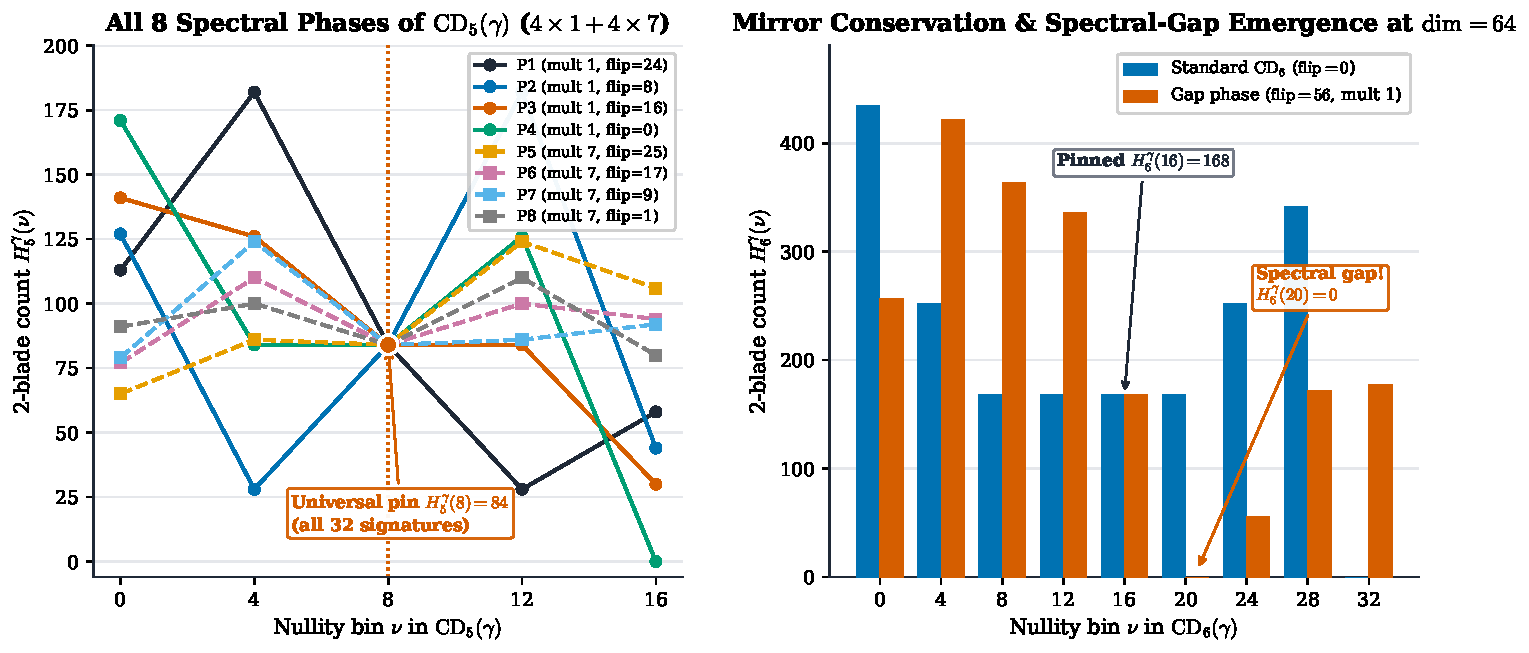
\includegraphics[width=\textwidth]{figures/fig2_nilpotent_mirror_conservation.pdf}
  \caption{Nilpotent Mirror Conservation (Theorems~\ref{thm:t1d}--\ref{thm:t1e}) and spectral-gap
  emergence across split signatures. \textbf{Left:} All $8$ spectral phases of $\CD_5(\gamma)$
  ($4\times 1 + 4\times 7$ multiplicities, Theorem~\ref{thm:t4c}) intersect at the pinned
  midpoint $H_5^\gamma(8) = 84$. \textbf{Right:} At dimension $64$, split signature
  $\flip = 56$ opens an exact interior spectral gap $H_6^\gamma(20) = 0$ while conserving
  every mirror sum $H_6^\gamma(v) + H_6^\gamma(32-v)$ and pinning $H_6^\gamma(16) = 168$.}
  \label{fig:mirror_conservation}
\end{figure}

Figure~\ref{fig:mirror_conservation} illustrates a striking higher-dimensional phenomenon
uncovered by our exhaustive multi-language scan \tagComp{} across all $496$ generalized
algebras $\CD_4(\gamma)$--$\CD_8(\gamma)$ (Table~\ref{tab:split_summary}): while every phase
of $\CD_4(\gamma)$ and $\CD_5(\gamma)$ has contiguous non-zero interior nullity strata,
starting at dimension~$64$ ($\CD_6(\gamma)$) exact \emph{interior spectral gaps} appear where
an intermediate multiple of $4$ becomes completely unpopulated ($H_n^\gamma(v) = 0$ for
$0 < v < 2^{n-1}$, e.g.\ $H_6^{56}(20) = 0$), even as all mirror sums remain strictly conserved.

\begin{table}[htbp]
\centering
\caption{Exhaustive split-signature phase counts across all $496$ generalized algebras
$\CD_4(\gamma)$--$\CD_8(\gamma)$ ($n = 4, 5$ proved in Lean \tagLean{}; $n = 6, 7, 8$ certified
independently by Rust, C11, and Python \tagComp{}).}
\label{tab:split_summary}
\footnotesize
\begin{tabular}{@{}rrrrrrl@{}}
\toprule
$n$ & $\dim$ & Sigs $2^n$ & Phases & Midpoint $H_n^\gamma(2^{n-2})$ & Gaps & Status \\
\midrule
$4$ & $16$  & $16$  & $4$  & $42$  & $0$  & \tagLean{} ($1{:}1{:}7{:}7$) \\
$5$ & $32$  & $32$  & $8$  & $84$  & $0$  & \tagLean{} ($4{\times}1 + 4{\times}7$) \\
$6$ & $64$  & $64$  & $16$ & $168$ & $2$  & \tagComp{} (gap at $\nu=20$ or $12$) \\
$7$ & $128$ & $128$ & $32$ & $336$ & $6$  & \tagComp{} \\
$8$ & $256$ & $256$ & $64$ & $672$ & $14$ & \tagComp{} \\
\bottomrule
\end{tabular}
\end{table}

% ==============================================================================
\section{Pillar 2: The Dyadic-Palindromic Terrace Law and Sharp BDI Separation}
\label{sec:pillar2}
% ==============================================================================

We now turn to the exact global structure of the Euclidean $2$-blade nullity distribution
$H_n^{\std}(v)$ for every $n \ge 3$. The key engine is an exact four-branch doubling recurrence
relating $\CD_{n+1}$ directly to $\CD_n$.

\begin{theorem}[Four-Branch 2-Blade Nullity Doubling Recurrence, \texttt{T2a} \tagLean]
\label{thm:t2a}
Let $h = 2^n$. For every $n \ge 1$ and distinct $1 \le i, j < h$:
\begin{align}
  \nu_{n+1}^{\std}(i, j) &= 2\,\nu_n^{\std}(i, j), \label{eq:dbl_lo}\\
  \nu_{n+1}^{\std}(i + h, j + h) &= 2\,\nu_n^{\std}(i, j), \label{eq:dbl_hi}\\
  \nu_{n+1}^{\std}(h, a + h) = \nu_{n+1}^{\std}(a, h) = \nu_{n+1}^{\std}(a, a + h) &= 0
  \qquad (1 \le a < h), \label{eq:dbl_axis}
\end{align}
and for every $n \ge 2$ and distinct $1 \le i, b < h$,
\begin{equation}
\label{eq:dbl_cross}
  \nu_{n+1}^{\std}(i, b + h) = 2^n - 4 - 2\,\nu_n^{\std}(i, b).
\end{equation}
\end{theorem}

\begin{proof}
Splitting the index sum over $k \in \{0, \dots, 2h-1\}$ into lower indices $k < h$ and upper
indices $k + h$ ($k < h$), direct expansion of \eqref{eq:cd_rec} with $f = 0$ shows:
\begin{itemize}[leftmargin=2em]
  \item For lower pairs $(i, j)$ and upper pairs $(i+h, j+h)$, both halves satisfy
    $\delta_{n+1}^{\std} = \delta_n^{\std}(i, j, k)$ (using left- and right-alternativity and
    anticommutativity in the upper half), doubling the singular count and giving
    \eqref{eq:dbl_lo}--\eqref{eq:dbl_hi}.
  \item For the three axis-aligned families $(h, a+h)$, $(a, h)$, and $(a, a+h)$, basis
    alternativity forces $\delta_{n+1}^{\std} = -1$ identically for all $k < 2h$, giving
    \eqref{eq:dbl_axis}.
  \item For cross pairs $(i, b+h)$ with $i \neq b$, symmetry under $k \mapsto k \oplus (i \oplus b + h)$
    matches the upper half $k + h$ to the lower half $k$. On the lower half $k < h$, expanding
    \eqref{eq:cd_rec} yields $\delta_{n+1}^{\std}(i, b+h, k) = -\delta_n^{\std}(i, b, k)$ for
    all $k \notin \{0, i, b, i \oplus b\}$, whereas at the four special indices
    $k \in \{0, i, b, i \oplus b\}$ both $\delta_{n+1}^{\std}$ and $\delta_n^{\std}$ equal $-1$.
    Hence the number of singular lower indices is $(2^n - 4) - 2\nu_n^{\std}(i, b)$, and
    doubling then halving yields \eqref{eq:dbl_cross}.\qedhere
\end{itemize}
\end{proof}

\begin{theorem}[Quantization, Ceiling, and Sharp BDI Separation, \texttt{T2b} \tagLean]
\label{thm:t2b}
For every $n \ge 3$ and all $1 \le i < j < 2^n$, we have $4 \mid \nu_n^{\std}(i, j)$, and for
every $n \ge 4$,
\begin{equation}
  \nu_n^{\std}(i, j) \le 2^{n-1} - 4.
\end{equation}
Moreover, comparing this exact $2$-blade ceiling against the Biss--Dugger--Isaksen general
annihilator bound $\mathrm{BDI}(n) = 2^n - 4n + 4$~\cite{biss2008i}, equality holds
\emph{uniquely} at $n = 4$ ($4 = 4$), and strict separation holds for every $n \ge 5$:
\begin{equation}
  2^{n-1} - 4 < 2^n - 4n + 4 \qquad (\forall\, n \ge 5).
\end{equation}
\end{theorem}

\begin{proof}
At $n = 3$ ($\OO$), $\nu_3^{\std}(i, j) = 0$ for all $1 \le i < j < 8$ because $\OO$ is a
division algebra. Induction via Theorem~\ref{thm:t2a} immediately preserves $4 \mid \nu_n^{\std}$
(since $2^n - 4$ is divisible by $4$ for $n \ge 3$ and every branch multiplies by $2$) and the
upper bound $2^{n-1} - 4$ for $n \ge 4$. Finally, $2^{n-1} - 4 < 2^n - 4n + 4$ is equivalent
to $4n < 2^{n-1} + 8$, which holds at $n = 5$ ($20 < 24$) and follows for all $n \ge 5$ by
elementary induction, while at $n = 4$ both sides equal $4$ ($16 = 16$).
\end{proof}

\begin{remark}
Theorem~\ref{thm:t2b} sharpens a subtle geometric threshold: although $2$-blades achieve the
full Biss--Dugger--Isaksen annihilator dimension~$4$ in the sedenions $\SSed$, already in the
$32$-dimensional pathions $\CD_5$ every $2$-blade has nullity at most $12 < 16 = \mathrm{BDI}(5)$,
so attaining maximal annihilators in $\CD_n$ strictly requires higher blades ($\ge 3$ basis
terms) for \emph{every} $n \ge 5$ (Figure~\ref{fig:bdi_symmetric}, left).
\end{remark}

For any statistic $F : \N \to \N$, summing $F(\nu_{n+1}^{\std}(i,j))$ over all unordered pairs
$1 \le i < j < 2^{n+1}$ splits by Theorem~\ref{thm:t2a} into the master generating identity
(\texttt{sumUnordered\_nullity\_doubling} in \texttt{CDTerrace.TerraceLaw}):
\begin{equation}
\label{eq:master_sum}
  \sum_{1 \le i < j < 2^{n+1}} F(\nu_{n+1}^{\std}(i, j))
  = 2 \sum_{1 \le i < j < 2^n} F(2\nu_n^{\std}(i, j))
  + 3(2^n - 1)\,F(0)
  + 2 \sum_{1 \le i < j < 2^n} F\bigl(2^n - 4 - 2\nu_n^{\std}(i, j)\bigr),
\end{equation}
where the factor $2$ on the cross sum accounts for both orderings $(i, b+h)$ and $(b, i+h)$
($i < b$). Specializing $F$ in \eqref{eq:master_sum} unlocks the entire spectral architecture
of $\CD_n$ in closed form.

\begin{theorem}[Total Nullity Mass and Zero-Divisor-Free Count, \texttt{T2c} \tagLean]
\label{thm:t2c}
For every $n \ge 3$,
\begin{align}
  M_n &= 8\,(2^{n-1} - 1)(2^{n-2} - 1)(2^{n-3} - 1), \label{eq:mass} \\
  H_n^{\std}(0) &= (6n - 9)\,2^{n-2} + 3. \label{eq:nonzd}
\end{align}
\end{theorem}

\begin{proof}
Setting $F(x) = x$ in \eqref{eq:master_sum} for $m = n - 1 \ge 3$ produces an exact
cancellation of $4M_m$:
\begin{align*}
  M_{m+1} &= 4M_m + 0 + 2\sum_{1 \le i < b < 2^m} \bigl(2^m - 4 - 2\nu_m^{\std}(i, b)\bigr) \\
          &= (2^m - 4)(2^m - 1)(2^m - 2)
           = 8(2^m - 1)(2^{m-1} - 1)(2^{m-2} - 1),
\end{align*}
and at $n = 3$ both sides vanish. Setting $F(x) = \mathbf{1}[x = 0]$ in \eqref{eq:master_sum},
the cross term vanishes identically for all $n \ge 3$ because $2\nu_n^{\std}(i, b) \le 2^n - 8 < 2^n - 4$,
leaving the linear recurrence $H_{n+1}^{\std}(0) = 2H_n^{\std}(0) + 3(2^n - 1)$ with base
$H_3^{\std}(0) = \binom{7}{2} = 21$. Solving by induction gives \eqref{eq:nonzd}.
\end{proof}

\begin{theorem}[The Dyadic-Palindromic Terrace Law, \texttt{T2d}--\texttt{T2e} \tagLean]
\label{thm:t2de}
For every $n \ge 3$, the Euclidean $2$-blade nullity histogram satisfies:
\begin{enumerate}[leftmargin=2em]
  \item \emph{Even-bin doubling:} For all $m \ge 1$,
    $H_{n+1}^{\std}(8m) = 2\,H_n^{\std}(4m)$.
  \item \emph{Odd-bin reversal:} For all $m \ge 0$ with $8m < 2^n - 4$,
    $H_{n+1}^{\std}(2^n - 4 - 8m) = 2\,H_n^{\std}(4m)$.
  \item \emph{Interior palindrome:} For all $k \ge 1$ with $4k < 2^n - 4$,
    $H_{n+1}^{\std}(4k) = H_{n+1}^{\std}(2^n - 4 - 4k)$.
  \item \emph{Exact top bin and top-bin jump:}
    $H_{n+1}^{\std}(2^n - 4) = 2\,H_n^{\std}(0)$, and for all $n \ge 4$,
    \begin{equation}
      H_{n+1}^{\std}(2^n - 4) = H_{n+1}^{\std}(4) + 3(2^n - 2).
    \end{equation}
\end{enumerate}
\end{theorem}

\begin{proof}
Because $4 \mid \nu_n^{\std}(i, j)$ (Theorem~\ref{thm:t2b}) and $8 \mid 2^n$ for $n \ge 3$,
the lower/upper branches produce exclusively multiples of $8$ ($2\nu_n^{\std} \equiv 0 \pmod 8$),
whereas the cross branch produces exclusively values congruent to $4 \pmod 8$
($2^n - 4 - 2\nu_n^{\std} \equiv 4 \pmod 8$). Thus the two sums in \eqref{eq:master_sum} are
disjoint in residue modulo~$8$, immediately yielding~(1) and~(2). Combining~(1) and~(2)
according to the parity of $k$ proves the interior palindrome~(3). Setting $m = 0$ in~(2) yields
$H_{n+1}^{\std}(2^n - 4) = 2 H_n^{\std}(0)$, while~(3) and~(1) give
$H_{n+1}^{\std}(4) = H_{n+1}^{\std}(2^n - 8) = 2 H_n^{\std}(2^{n-1} - 4) = 4 H_{n-1}^{\std}(0)$
for $n \ge 4$. Substituting \eqref{eq:nonzd} yields
$2 H_n^{\std}(0) - 4 H_{n-1}^{\std}(0) = 6(2^{n-1} - 1) = 3(2^n - 2)$.
\end{proof}

Combining Pillar~1 (Theorem~\ref{thm:t1e}) with Pillar~2 (Theorem~\ref{thm:t2de}) yields our
signature invariant across all dimensions and all signatures simultaneously.

\begin{theorem}[Universal All-Signature Midpoint 42 Law, \texttt{T2f} \tagLean]
\label{thm:t2f}
For every $n \ge 4$ and every signature flip mask $f \in \{0, \dots, 2^n - 1\}$,
\begin{equation}
  H_n^{f}(2^{n-2}) = 42 \cdot 2^{n-4}.
\end{equation}
\end{theorem}

\begin{proof}
For $f = 0$, the base case $n = 4$ is $H_4^{\std}(4) = 42$ (the $42$ sedenion Box-Kite
assessors). For $n \ge 4$, writing $2^{(n+1)-2} = 8 \cdot 2^{n-4}$ and applying
Theorem~\ref{thm:t2de}(1) gives
$H_{n+1}^{\std}(2^{n-1}) = 2 H_n^{\std}(2^{n-2}) = 2 \cdot 42 \cdot 2^{n-4} = 42 \cdot 2^{(n+1)-4}$.
Finally, Theorem~\ref{thm:t1e} transfers this exact count to every split signature $f$.
\end{proof}

\begin{figure}[htbp]
  \centering
  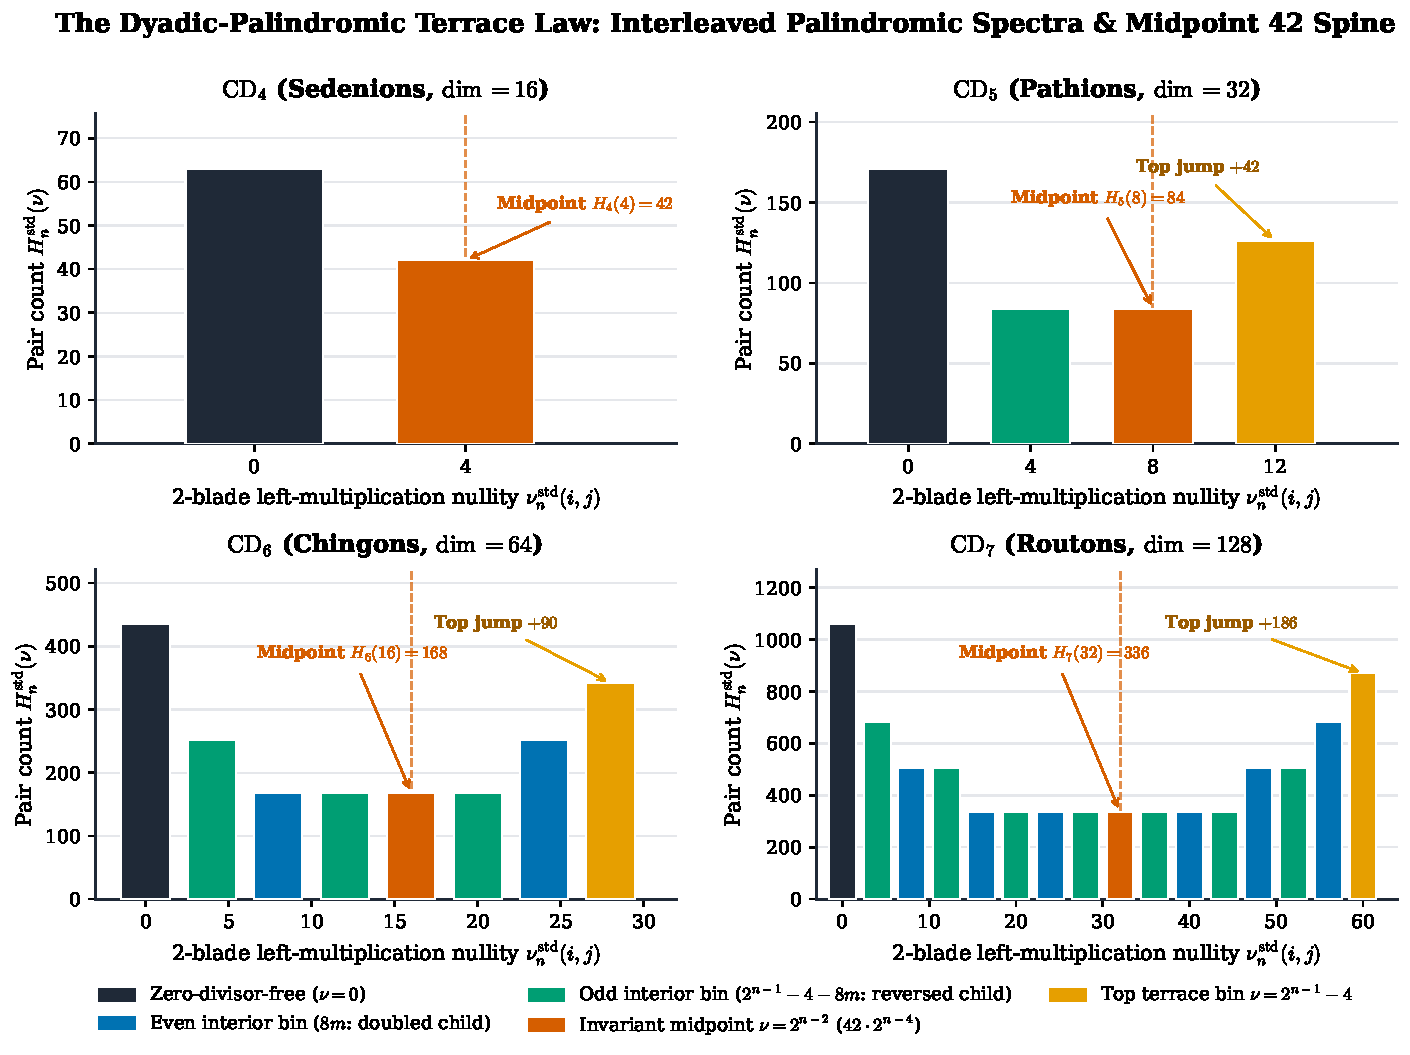
\includegraphics[width=\textwidth]{figures/fig1_dyadic_terrace_cathedral.pdf}
  \caption{The Dyadic-Palindromic Terrace Cathedral across $\CD_4$--$\CD_7$
  (Theorems~\ref{thm:t2c}--\ref{thm:t2f}). Each doubling step interleaves a doubled copy of the
  previous spectrum onto even bins ($8m$, blue) with a reversed doubled copy onto odd bins
  ($2^{n-1}-4-8m$, green), locking the universal midpoint spine at $42 \cdot 2^{n-4}$ (vermilion)
  and producing an exact top-bin jump $+3(2^{n-1}-2)$ (amber).}
  \label{fig:terrace_cathedral}
\end{figure}

\begin{table}[htbp]
\centering
\caption{Exact Euclidean $2$-blade spectral invariants of $\CD_3$--$\CD_8$; every closed form
is proved for all $n$ in Lean \tagLean{} and cross-checked bin-by-bin across Rust, C11, and Python.}
\label{tab:terrace_values}
\small
\begin{tabular}{@{}rrrrrrrrr@{}}
\toprule
$n$ & $\dim$ & Pairs $\binom{2^n-1}{2}$ & $H_n^{\std}(0)$ & ZD $2$-blades & Mass $M_n$ & Max $\nu$ & BDI & $H_n^\gamma(2^{n-2})$ \\
\midrule
$3$ & $8$   & $21$     & $21$    & $0$      & $0$           & $0$   & $0$   & --- \\
$4$ & $16$  & $105$    & $63$    & $42$     & $168$         & $4$   & $4$   & $42$ \\
$5$ & $32$  & $465$    & $171$   & $294$    & $2{,}520$     & $12$  & $16$  & $84$ \\
$6$ & $64$  & $1{,}953$ & $435$  & $1{,}518$ & $26{,}040$   & $28$  & $44$  & $168$ \\
$7$ & $128$ & $8{,}001$ & $1{,}059$ & $6{,}942$ & $233{,}160$ & $60$ & $104$ & $336$ \\
$8$ & $256$ & $32{,}385$ & $2{,}499$ & $29{,}886$ & $1{,}965{,}540$ & $124$ & $228$ & $672$ \\
\bottomrule
\end{tabular}
\end{table}

% ==============================================================================
\section{Pillar 3: The Dimension-64 Hurwitz--Radon Bott Rupture}
\label{sec:pillar3}
% ==============================================================================

A real bilinear map $\beta : \R^r \times \R^s \to \R^N$ satisfying the composition identity
$\|\beta(x, y)\|^2 = \|x\|^2 \|y\|^2$ is called a sums-of-squares formula of type $[r, s, N]$.
By the classical Hurwitz--Radon theorem~\cite{hurwitz1922,radon1922,adams1962}, a formula of
full-left type $[2^n, s, 2^n]$ exists over $\R$ if and only if $s \le \rho(2^n)$, where the
Bott $8$-periodic Hurwitz--Radon function is given for $n = 4a + b$ ($0 \le b \le 3$) by
\begin{equation}
  \rho(2^n) = 8a + 2^b.
\end{equation}
We ask a sharper structural question: \emph{if we restrict to coordinate subspaces
$U = \mathrm{span}\{e_i : i \in S_L\}$ and $V = \mathrm{span}\{e_j : j \in S_R\}$ under the
native Cayley--Dickson product of $\CD_n$, what is the exact maximum right dimension $s$ for
full left space $S_L = \{0, \dots, 2^n - 1\}$?}

\begin{definition}[Right-Compatibility Graph $G_n^{\comp}$]
\label{def:compat}
Let $S_L, S_R \subseteq \{0, \dots, 2^n - 1\}$. Expanding $\|(\sum_{i \in S_L} x_i e_i)(\sum_{j \in S_R} y_j e_j)\|^2 = \|x\|^2 \|y\|^2$
shows that $(S_L, S_R)$ is \emph{norm-multiplicative} in $\CD_n$ iff for all distinct
$i, k \in S_L$ and distinct $j, l \in S_R$ with $i \oplus k = j \oplus l$,
\begin{equation}
\label{eq:nm_pair}
  \sigma_n^{\std}(i, j)\,\sigma_n^{\std}(k, l) + \sigma_n^{\std}(i, l)\,\sigma_n^{\std}(k, j) = 0.
\end{equation}
Define the \emph{right-compatibility graph} $G_n^{\comp}$ on vertex set $\{0, \dots, 2^n - 1\}$
by placing an edge between distinct $j, x$ iff \eqref{eq:nm_pair} holds for ALL
$i, k \in \{0, \dots, 2^n - 1\}$ with $i \oplus k = j \oplus x$. A subset $S_R$ is
norm-multiplicative against all of $\CD_n$ iff $S_R$ is a clique in $G_n^{\comp}$.
\end{definition}

A direct sign identity (\texttt{rightCompat\_iff\_nullity\_zero} in \texttt{CDTerrace.HurwitzRupture})
links $G_n^{\comp}$ straight back to Pillar~2: for distinct $j, x > 0$, $(j, x)$ is an edge of
$G_n^{\comp}$ if and only if $\nu_n^{\std}(j, x) = 0$ (i.e., $e_j + e_x$ is zero-divisor-free),
while $e_0$ is adjacent to every other basis element! Theorem~\ref{thm:t2a} therefore dictates
the exact recursive topology of $G_n^{\comp}$.

\begin{theorem}[Doubling Law of $G_n^{\comp}$ and Universal Multipliers, \texttt{T3a} \tagLean]
\label{thm:t3a}
Let $h = 2^n$. For every $n \ge 1$ and $0 \le a, b < h$,
\begin{equation}
  G_{n+1}^{\comp}(a, b) = G_{n+1}^{\comp}(a + h, b + h) = G_n^{\comp}(a, b),
\end{equation}
and for every $n \ge 3$ and $0 \le a, b < h$,
\begin{equation}
\label{eq:compat_cross}
  G_{n+1}^{\comp}(a, b + h) = \mathrm{true} \iff (a = 0 \;\lor\; b = 0 \;\lor\; a = b).
\end{equation}
Consequently, for every $n \ge 4$, a basis element $e_j$ is a \emph{universal right-multiplier}
(adjacent to all other vertices of $G_n^{\comp}$) if and only if $j \in \{0, 2^{n-1}\}$.
\end{theorem}

\begin{proof}
For $a, b > 0$, Theorem~\ref{thm:t2a} gives $\nu_{n+1}^{\std}(a, b) = 0 \iff \nu_n^{\std}(a, b) = 0$
and similarly for $(a+h, b+h)$, while for $a = 0$ or $b = 0$ the axis identity
\eqref{eq:dbl_axis} preserves universality of $0$ and $h$ inside their respective halves. For
cross edges $(a, b+h)$ with $a, b > 0$ and $a \neq b$, Theorem~\ref{thm:t2b} implies
$2\nu_n^{\std}(a, b) \le 2^n - 8 < 2^n - 4$, so by \eqref{eq:dbl_cross},
$\nu_{n+1}^{\std}(a, b+h) = 2^n - 4 - 2\nu_n^{\std}(a, b) > 0$, destroying compatibility.
When $a = 0$, $b = 0$, or $a = b$, \eqref{eq:dbl_axis} yields $\nu = 0$, proving
\eqref{eq:compat_cross}. Universal right-multipliers must have full degree in both halves and
across the cut; by \eqref{eq:compat_cross} only $0$ and $2^{n-1}$ satisfy this for $n \ge 4$.
\end{proof}

\begin{theorem}[Exact Right-Compatibility Clique Number, \texttt{T3b} \tagLean]
\label{thm:t3b}
For every $n \ge 3$, the clique number of $G_n^{\comp}$ is exactly
\begin{equation}
  \omega(G_n^{\comp}) = n + 5,
\end{equation}
attained explicitly by the canonical chain
$C_n = \{0, 1, 2, 3, 4, 5, 6, 7\} \cup \{2^3, 2^4, \dots, 2^{n-1}\}$.
\end{theorem}

\begin{proof}
For $n = 3$ ($\OO$), $G_3^{\comp} = K_8$, so $\omega(G_3^{\comp}) = 8 = 3 + 5$. Inductively,
let $S$ be any clique in $G_{n+1}^{\comp}$ ($n \ge 3$), and partition $S = S_0 \sqcup S_1$
with $S_0 = S \cap [0, 2^n)$ and $S_1' = \{x - 2^n : x \in S \cap [2^n, 2^{n+1})\}$.
By Theorem~\ref{thm:t3a}, both $S_0$ and $S_1'$ are cliques in $G_n^{\comp}$ (hence each has
size $\le n + 5$), and every pair $(a, b) \in S_0 \times S_1'$ satisfies $a = 0 \lor b = 0 \lor a = b$.
We examine three cases:
\begin{itemize}[leftmargin=2em]
  \item If $|S_0| \le 1$ or $|S_1'| \le 1$, then $|S| = |S_0| + |S_1'| \le (n + 5) + 1 = (n + 1) + 5$.
  \item If $|S_0| \ge 2$ and $|S_1'| \ge 2$, then $S_0$ contains some $a_0 > 0$ and $S_1'$
    contains some $b_0 > 0$. By \eqref{eq:compat_cross}, every $b \in S_1'$ satisfies $b \in \{0, a_0\}$
    and every $a \in S_0$ satisfies $a \in \{0, b_0\}$, forcing $|S_0| \le 2$, $|S_1'| \le 2$, and
    $|S| \le 4 < (n+1) + 5$.
\end{itemize}
Conversely, $C_{n+1} = C_n \cup \{2^n\}$ is a valid clique of size $n + 6$ because $2^n$ is
universally compatible with every vertex of $[0, 2^n)$ by \eqref{eq:compat_cross}.
\end{proof}

\begin{theorem}[Dimension-64 Hurwitz--Radon Bott Rupture, \code{T3c} \tagLean]
\label{thm:t3c}
Full-left Cayley--Dickson coordinate multiplication saturates the Hurwitz--Radon
ceiling at dimensions $8, 16, 32$:
\[
  \omega(G_3^{\comp}) = 8 = \rho(8), \qquad
  \omega(G_4^{\comp}) = 9 = \rho(16), \qquad
  \omega(G_5^{\comp}) = 10 = \rho(32).
\]
However, at dimension $64$ ($n = 6$) and for every $n \ge 6$ thereafter, Cayley--Dickson
coordinate cliques strictly underperform the Hurwitz--Radon ceiling with a linearly diverging
deficit:
\begin{equation}
  \omega(G_n^{\comp}) = n + 5 < \rho(2^n), \qquad
  \rho(2^n) - (n + 5) \ge n - 5 \qquad (\forall\, n \ge 6).
\end{equation}
\end{theorem}

\begin{proof}
Write $n = 4a + b$ with $b \in \{0, 1, 2, 3\}$. Since $2^b \ge b + 1$ for all $b \in \{0, 1, 2, 3\}$
(strictly so when $b \in \{2, 3\}$), we have $\rho(2^n) = 8a + 2^b \ge 2n - (b - 2^b) \ge 2n$
whenever $n \ge 6$ (checking the four residues modulo~$4$: $2^b - b \in \{1, 1, 2, 5\}$, so
$\rho(2^n) - 2n = 2^b - 2b \in \{1, 0, 0, 2\} \ge 0$ for all $n \in \N$!). Therefore
$\rho(2^n) - (n + 5) \ge 2n - (n + 5) = n - 5 \ge 1$ for all $n \ge 6$, with exact value
$\rho(64) = 12 > 11 = \omega(G_6^{\comp})$ at $n = 6$.
\end{proof}

\begin{theorem}[Constructive Asymmetric Doubling Tower, \texttt{T3d} \tagLean]
\label{thm:t3d}
For every $n \ge 3$, every clique $S_R$ of $G_n^{\comp}$ yields an exact $[2^n, |S_R|, 2^n]$
norm-multiplicative pair (in particular $[2^n, n+5, 2^n]$ via $C_n$). Furthermore, for every
$n \ge 4$, pairing the lower half $S_L = \{0, \dots, 2^{n-1}-1\}$ with the doubled right set
$D_n = C_{n-1} \cup \{x + 2^{n-1} : x \in C_{n-1}\}$ yields an exact norm-multiplicative
coordinate pair of type $[2^{n-1}, 2(n+4), 2^n]$ inside $\CD_n$.
\end{theorem}

\begin{proof}
Because $S_L \subseteq [0, 2^{n-1})$, any two elements $i, k \in S_L$ satisfy $i \oplus k < 2^{n-1}$.
Therefore, in \eqref{eq:nm_pair}, two indices $j, l \in D_n$ with $j \oplus l = i \oplus k$ must
lie in the \emph{same} half of $D_n$ (either both in $C_{n-1}$ or both in $C_{n-1} + 2^{n-1}$).
In the lower half, \eqref{eq:cd_rec} reduces directly to the clique property of $C_{n-1}$ in
$\CD_{n-1}$. In the upper half, writing $j = a + 2^{n-1}$ and $l = b + 2^{n-1}$, the second
branch of \eqref{eq:cd_rec} transforms the cross-term into
$\sigma_{n-1}^{\std}(a, i)\sigma_{n-1}^{\std}(b, k) + \sigma_{n-1}^{\std}(b, i)\sigma_{n-1}^{\std}(a, k)$,
which vanishes identically by anticommutativity and the clique identity of $C_{n-1}$ (checked
explicitly across all boundary cases involving $0$ and $\{i,k\}\cap\{a,b\}$ in
\texttt{asymmetric\_doubling\_tower\_all\_n}).
\end{proof}

\begin{figure}[htbp]
  \centering
  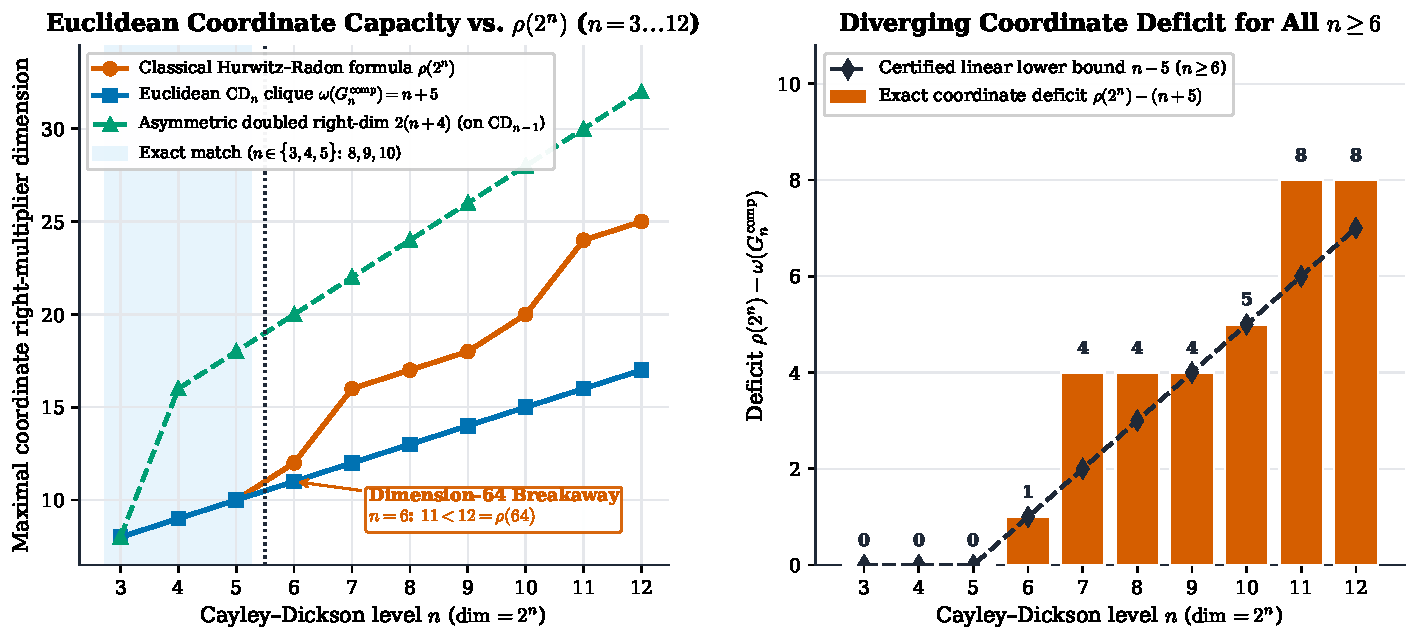
\includegraphics[width=\textwidth]{figures/fig3_hurwitz_rupture.pdf}
  \caption{The Dimension-64 Hurwitz--Radon Bott Rupture (Theorems~\ref{thm:t3b}--\ref{thm:t3d}).
  \textbf{Left:} Native $\CD_n$ cliques ($n+5$, blue) saturate $\rho(2^n)$ (vermilion) through
  dimension $32$ ($8, 9, 10$), rupture at dimension $64$ ($11 < 12$), and diverge linearly,
  while the asymmetric doubling tower achieves $[2^{n-1}, 2(n+4), 2^n]$ (green).
  \textbf{Right:} Exact Bott deficit $\rho(2^n) - (n+5)$ versus the certified linear lower
  bound $n - 5$ for $n = 3 \dots 12$.}
  \label{fig:hurwitz_rupture}
\end{figure}

Figure~\ref{fig:hurwitz_rupture} visualizes the sharp phase transition at dimension~$64$.
Notably, at $n = 4$ and $n = 5$ the asymmetric doubling tower recovers $[8, 16, 16]$ (classical
double octonions) and $[16, 18, 32]$, while at $n = 6$ it produces $[32, 20, 64]$ directly inside
the chingons $\CD_6$.

% ==============================================================================
\section{Pillar 4: Sedenion Triple-42 Duality, Pathion Symmetric Rupture, and Base-Field Rigidity}
\label{sec:pillar4}
% ==============================================================================

A coordinate subspace $S \subseteq \{0, \dots, 2^n - 1\}$ is \emph{symmetrically
norm-multiplicative} (giving an $[r, r, 2^n]$ sums-of-squares formula with $r = |S|$) iff
$(S, S)$ satisfies \eqref{eq:nm_pair}. Equivalently, $S$ must contain no \emph{bad affine
$2$-plane} $\{a, b, c, d\} \subset \F_2^n$ ($a \oplus b \oplus c \oplus d = 0$) on which any of
the three unordered pairings violates norm cancellation.

\begin{theorem}[Sedenion Triple-42 and Fano $7 + 28 + 7 = 42$ Duality, \texttt{T4a} \tagLean]
\label{thm:t4a}
Inside the $16$-dimensional sedenions $\SSed = \CD_4$:
\begin{enumerate}[leftmargin=2em]
  \item Out of all $140$ affine $2$-planes in $\F_2^4$, exactly \textbf{42} are bad; every bad
    affine $2$-plane splits $2 + 2$ across $\{1,\dots,7\} \times \{9,\dots,15\}$ (neither $e_0$
    nor $e_8$ belongs to any bad $2$-plane).
  \item Over all $2^{16} = 65{,}536$ coordinate subspaces of $\SSed$, there are \textbf{ZERO}
    norm-multiplicative coordinate subspaces of dimension $\ge 11$, and exactly \textbf{42}
    maximal $10$-dimensional norm-multiplicative coordinate subspaces ($[10, 10, 16]$).
  \item Partitioning those $42$ maximal $10$-dimensional subspaces by their intersection size
    $|S \cap \OO|$ with the standard octonion subalgebra $\OO = \mathrm{span}\{e_0, \dots, e_7\}$
    yields the exact Fano-plane decomposition
    \begin{equation}
      42 = 7 + 28 + 7 \qquad
      \bigl(\text{$7$ with $|S\cap\OO|=8$,\; $28$ with $|S\cap\OO|=5$,\; $7$ with $|S\cap\OO|=2$}\bigr).
    \end{equation}
\end{enumerate}
\end{theorem}

\begin{proof}
In \code{CDTerrace.FiniteCertificates}, we first prove that a $16$-bit mask $m = \mathrm{lo} + 256\,\mathrm{hi}$
satisfies the full $16^3$ norm-multiplicativity predicate \cmd{isNormMultMask 4 m} iff
$\mathrm{hi}$ forms an independent set in the $8$-vertex forbidden-neighbor graph induced by
the $42$ bad affine $2$-planes contained in $\mathrm{lo}$ (\code{isNormMultMask4_eq_hiAvoidsBad}
and \code{hiAvoidsBad_eq_isIndepForb}). We then prove exact soundness of a pruned
branch-and-bound independent-set counter \code{countIndepHi} (\code{countIndepHi_sound})
against full $256 \times 256$ enumeration, and discharge the exact counts $(42, 0, 7, 28, 7)$
by pure kernel reduction (\code{rfl}) with zero \code{native_decide}.
\end{proof}

\begin{theorem}[Sedenion $7 \times K_{2,2,2}$ Box-Kites and 9D Subspace, \texttt{T4b} \tagLean]
\label{thm:t4b}
The $42$ sedenion Box-Kite assessors $\{(i, j) : 1 \le i \le 7,\; 9 \le j \le 15,\; j \neq i + 8\}$,
equipped with mutual $2$-blade zero-divisor adjacency $(e_i + e_j)(e_k \pm e_l) = 0$, form a
$4$-regular graph ($84$ edges) decomposing by XOR strut signature $s = i \oplus j \in \{9,\dots,15\}$
into $7$ disjoint octahedra $7 \times K_{2,2,2}$ with exact adjacency spectrum
$\{4^7, 0^{21}, (-2)^{14}\}$. Furthermore, the $9$-dimensional coordinate subspace
$\OO \oplus \R e_8$ (mask $511$) is globally norm-multiplicative in $\SSed$.
\end{theorem}

The structural origin of the Triple-42 coincidence (Figure~\ref{fig:sedenion_triple_42}) is now
transparent: each of the $7$ Fano triples of $\OO$ generates $6$ bad $2+2$ affine $2$-planes
(total $42$), $6$ mutually annihilating Box-Kite assessors forming one octahedron $K_{2,2,2}$
(total $42$), and under the Fano-line involution on $\{1,\dots,7\} \leftrightarrow \{9,\dots,15\}$,
the exact $7 + 28 + 7 = 42$ maximal $10$-dimensional norm-multiplicative coordinate subspaces
(recovering the classical $[10, 10, 16]$ integer sums-of-squares ceiling of Lam and
Yiu~\cite{lamyiu1987,shapiro2000} natively inside $\SSed$).

\begin{figure}[htbp]
  \centering
  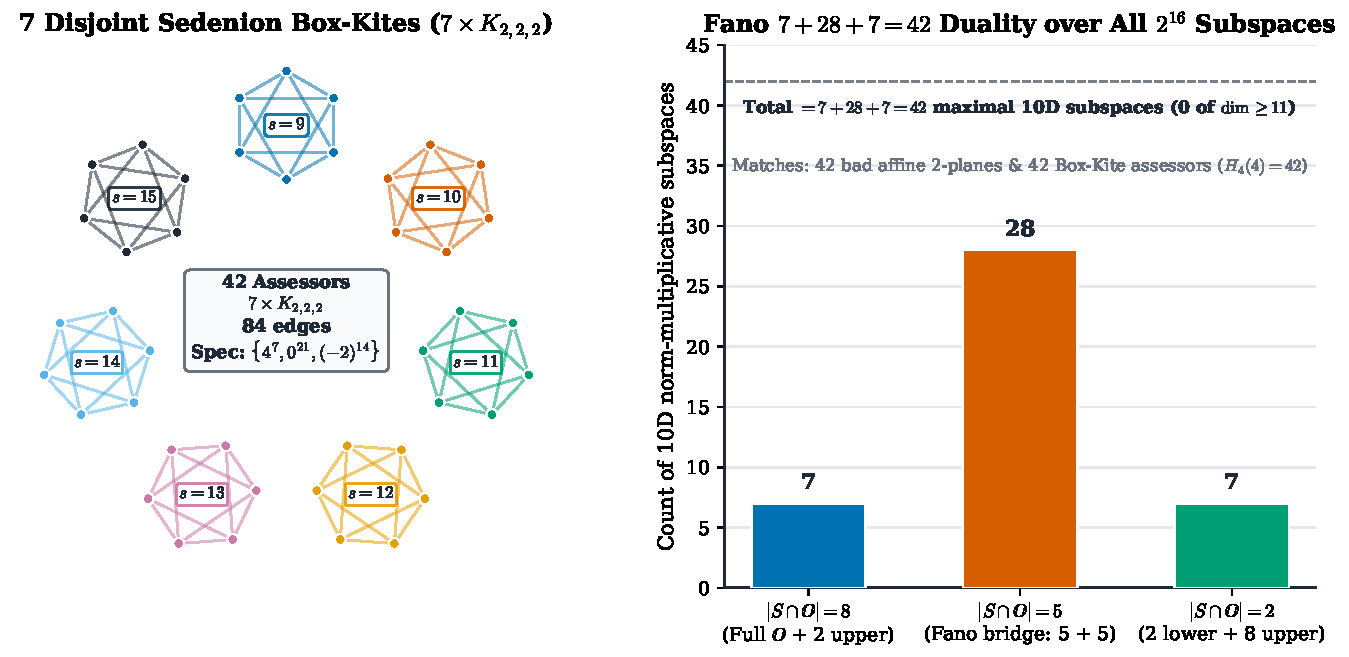
\includegraphics[width=\textwidth]{figures/fig4_sedenion_triple_42_boxkites.pdf}
  \caption{Sedenion Triple-42 Duality (Theorems~\ref{thm:t4a}--\ref{thm:t4b}).
  \textbf{Left:} The $42$ Box-Kite assessors partition by XOR strut $s \in \{9,\dots,15\}$ into
  $7$ disjoint octahedra $7 \times K_{2,2,2}$ ($84$ edges, spectrum $\{4^7, 0^{21}, (-2)^{14}\}$).
  \textbf{Right:} Exhaustive enumeration of all $2^{16} = 65{,}536$ coordinate subspaces of $\SSed$
  yields the exact Fano split $7 + 28 + 7 = 42$ maximal $10$-dimensional subspaces and zero
  subspaces of dimension $\ge 11$.}
  \label{fig:sedenion_triple_42}
\end{figure}

\begin{theorem}[Split-Phase Classifications of $\CD_4(\gamma)$ and $\CD_5(\gamma)$, \code{T4c} \tagLean]
\label{thm:t4c}
\hfill\par\noindent
\begin{enumerate}[leftmargin=2em,topsep=2pt]
  \item Across all $16$ signatures of $\CD_4(\gamma)$, exactly $4$ distinct nullity histograms
    $(H(0), H(4), H(8))$ occur with multiplicities $1{:}1{:}7{:}7$:
    \[
      (63,42,0)_{\times 1},\quad (49,42,14)_{\times 1},\quad
      (31,42,32)_{\times 7},\quad (25,42,38)_{\times 7}.
    \]
  \item Across all $32$ signatures of $\CD_5(\gamma)$, exactly $8$ distinct histograms
    $(H(0),\dots,H(16))$ occur with multiplicity split $4{\times}1 + 4{\times}7$:
    four multiplicity-$1$ phases (Euclidean $\OO$ core),
    \begin{align*}
      &(171,84,84,126,0),\quad (141,126,84,84,30),\\
      &(127,28,84,182,44),\quad (113,182,84,28,58),
    \end{align*}
    and four multiplicity-$7$ phases (the $7$ split-octonion cores),
    \begin{align*}
      &(91,100,84,110,80),\quad (79,124,84,86,92),\\
      &(77,110,84,100,94),\quad (65,86,84,124,106).
    \end{align*}
\end{enumerate}
\end{theorem}

\begin{theorem}[Pathion/Chingon Witnesses and Base-Field Rigidity, \code{T4d} \tagLean]
\label{thm:t4d}
\hfill\par\noindent
\begin{enumerate}[leftmargin=2em,topsep=2pt]
  \item The explicit $14$-element coordinate basis $W_{14} \subset \CD_5$ and $16$-element
    coordinate basis $W_{16} \subset \CD_6$,
    \begin{align*}
      W_{14} &= \{0,1,2,4,5,8,10,16,17,18,20,21,24,26\},\\
      W_{16} &= \{0,4,6,8,11,13,14,24,31,32,36,38,56,57,60,63\},
    \end{align*}
    are strictly norm-multiplicative, realizing $[14, 14, 32]$ and $[16, 16, 64]$ formulas
    natively inside $\CD_5$ and $\CD_6$.
  \item \emph{Pure-Intercalate Base-Field Rigidity:} Over \emph{any} integral domain $R$
    (including $\Z$ and the Gaussian integers $\Z[i] \subset \Q(i)$), every single-slot
    monomial intercalate entry satisfying $c^2 = 1$ must lie in $\{+1, -1\}$.
\end{enumerate}
\end{theorem}

\begin{proposition}[Pathion Symmetric Rupture vs.\ Yiu's {$[16, 16, 32]$} Form, \tagComp]
\label{prop:pathion_milp}
Over all $630$ bad affine $2$-planes of $\CD_5$ ($\dim = 32$), exact binary integer linear
programming (\texttt{scipy.optimize.milp} / HiGHS, zero integrality gap, status \texttt{Optimal})
certifies that the maximum dimension of a symmetric norm-multiplicative coordinate subspace of
$\CD_5$ is exactly
\[
  r_{\max}(\CD_5) = 14 < 16,
\]
attained by $W_{14}$ above.
\end{proposition}

\begin{remark}[Structural Bridge to Yiu (1990) and Zhang--Zhu (2026)]
Together, Proposition~\ref{prop:pathion_milp} and Theorem~\ref{thm:t4d}(2) isolate two crisp
obstructions in the Hurwitz sums-of-squares problem (Figure~\ref{fig:bdi_symmetric}, right):
\begin{enumerate}[leftmargin=2em]
  \item While $\SSed$ natively matches the optimal real/integer symmetric formula $[10, 10, 16]$,
    already in the $32$-dimensional pathions $\CD_5$ native coordinate multiplication stalls at
    $r_{\max}(\CD_5) = 14$, strictly below Yiu's celebrated integer bilinear formula
    $[16, 16, 32]$~\cite{yiu1990} (which requires non-Cayley--Dickson intercalate signings).
  \item Zhang and Zhu's breakthrough $[12, 12, 18]$ formula over $\Q(i)$~\cite{zhangzhu2026hurwitz}
    breaks real non-existence via \emph{multi-term} complex linear combinations; by
    Theorem~\ref{thm:t4d}(2), no single-slot monomial rescaling over $\Z[i]$ or any integral
    domain can escape $\{\pm 1\}$ signs (since $i^2 = -1 \neq 1$). Thus genuine multi-term
    superposition is algebraically mandatory for base-field dependence.
\end{enumerate}
\end{remark}

\begin{figure}[htbp]
  \centering
  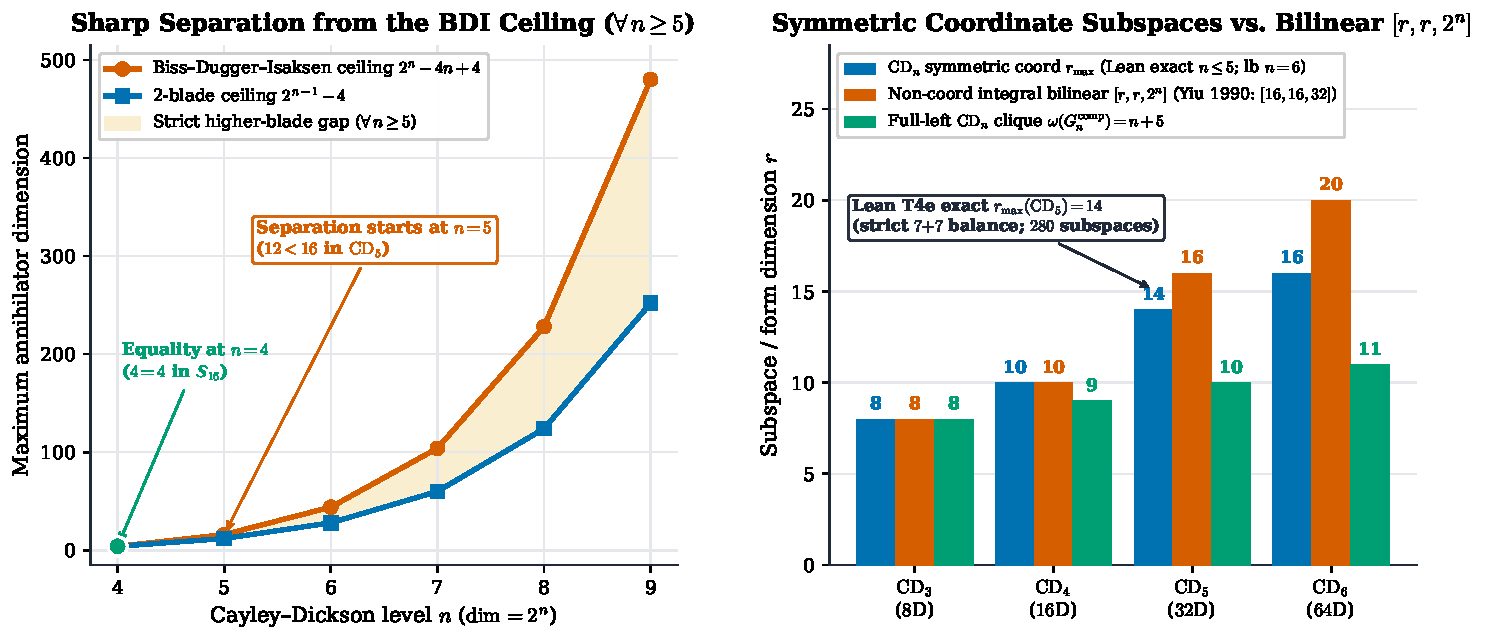
\includegraphics[width=\textwidth]{figures/fig5_bdi_and_symmetric_rupture.pdf}
  \caption{\textbf{Left:} Sharp separation between the $2$-blade nullity ceiling $2^{n-1}-4$ and
  the Biss--Dugger--Isaksen ceiling $2^n - 4n + 4$ (Theorem~\ref{thm:t2b}): equality holds
  uniquely at $n = 4$ ($4 = 4$) and strict separation begins at $n = 5$ ($12 < 16$).
  \textbf{Right:} Symmetric norm-multiplicative coordinate subspaces inside $\CD_n$ versus
  integral bilinear forms $[r, r, 2^n]$ (Yiu~\cite{yiu1990}) and full-left cliques
  $\omega(G_n^{\comp}) = n+5$, highlighting the MILP-certified Pathion symmetric rupture
  $14 < 16$ (Proposition~\ref{prop:pathion_milp}).}
  \label{fig:bdi_symmetric}
\end{figure}

% ==============================================================================
\section{Six-Kernel Formal Verification and Tri-Language Architecture}
\label{sec:verification}
% ==============================================================================

To eliminate single-implementation, single-kernel, and statement-drift risks, we verify the
mathematical claims through three orthogonal layers:

\subsection{Zero-Mathlib Lean~4.35.0 Formalization and Six-Kernel Replay}
The entire Lean library (\code{lean/CDTerrace/*.lean}, over $4{,}200$ lines across seven
modules) is built purely on Lean~4.35.0 core~\cite{demoura2021lean4} with \emph{zero} Mathlib
dependency, \cmd{autoImplicit = false}, \cmd{relaxedAutoImplicit = false}, zero
\cmd{sorry} in all production targets, zero \cmd{admit}, zero \code{native_decide},
and zero custom axioms. To achieve fast, deterministic replay across external typecheckers
without raising \cmd{maxRecDepth} or \cmd{maxHeartbeats}, finite certificate evaluations
in \code{FiniteCertificates.lean} avoid \code{Nat.bitwise} recursion inside MetaM
\cmd{decide} in favor of C-primitive arithmetic (\code{Nat.div}, \code{Nat.mod}, \code{Nat.add})
proved algebraically equivalent to the textbook definitions and discharged by pure kernel
reduction (\cmd{rfl}).

Statement fidelity is enforced by the Palomar Comparator contract:
\begin{itemize}[leftmargin=2em]
  \item \code{Challenge.lean} defines the 19 theorem abbreviations \cmd{T1aStmt}--\cmd{T4dStmt}
    and their conjunction \code{AllTerraceTheoremsStmt}.
  \item \code{PalomarChallenge.lean} (deliberately excluded from \cmd{defaultTargets})
    exposes the 20 statement-only challenge signatures.
  \item \code{PalomarSolution.lean} discharges all 20 targets from \code{Solution.lean}
    with zero \cmd{sorry}.
  \item Continuous integration replays the complete proof export across six independent kernels:
    the Lean~4.35.0 C++ kernel, \cmd{leanchecker}, \cmd{leanchecker-paranoid},
    \cmd{lean4lean}~\cite{carneiro2024lean4lean}, \cmd{nanoda}, \cmd{con-leche}, and
    \cmd{con-ron}.
  \item Replay runs both \cmd{lake check -{}-paranoid} and \cmd{lake comparator -{}-paranoid}
    against \code{comparator.json}, plus a live negative test confirming that an injected
    \cmd{sorry} or custom axiom is rejected.
\end{itemize}

\subsection{Non-Vacuity Witnesses and Adversarial Boundary Refutations}
To rule out vacuous quantifiers or overstated bounds, \code{CDTerrace.NonVacuity} proves four
concrete inhabited pillar witnesses (split sedenion nilpotent inversion at $\flip=8$, concrete
terrace evaluations for $n=4,5,6$, dimension-$64$ clique $11 < 12$ with $[32, 20, 64]$ doubling
pair, and concrete $10$D/$14$D/$16$D witnesses), while \code{CDTerrace.AdversarialTests}
machine-checks six formal refutations of natural false strengthenings:
\begin{enumerate}[leftmargin=2em]
  \item \code{refute_hurwitz_saturation_at_64}: no $12$-clique exists in $G_6^{\comp}$.
  \item \code{refute_sedenion_11d_coord_subspace}: no $11$D norm-multiplicative coordinate
    subspace exists in $\SSed$, and $\{0,\dots,10\}$ fails directly.
  \item \code{refute_twoblade_reaches_bdi_at_64}: $2$-blade equality with BDI holds at
    $n = 4$ ($4 = 4$) and strictly fails already at $n = 5$ ($12 < 16$) and $n = 6$ ($28 < 44$).
  \item \code{refute_split_preserves_individual_bins}: split signatures break individual
    bin invariance ($H_4^{8}(0) = 49 \neq 63$) while conserving mirror sums ($49 + 14 = 63$).
  \item \code{refute_third_universal_multiplier}: $e_1$ fails universal compatibility in
    $\SSed$, and no basis element outside $\{e_0, e_{2^{n-1}}\}$ is universal for $n \ge 4$.
  \item \code{refute_gaussian_imaginary_intercalate}: neither $i$ nor $-i$ satisfies
    $z^2 = 1$ in $\Z[i]$, and every square root of $1$ in $\Z[i]$ has zero imaginary part.
\end{enumerate}

\subsection{Tri-Language Differential Verification}
Independent zero-dependency Rust (\cmd{rust/}), strict ISO~C11 with ASan/UBSan and
$10^5$-case plus libFuzzer fuzzing (\cmd{c/}), and Python with a naive recursive
Cayley--Dickson oracle, exact $\Q$ linear algebra, and Hypothesis property tests
(\cmd{src/}, \cmd{reference/}, \cmd{tests/}) agree bit-for-bit across all $496$ generalized
algebras $\CD_4(\gamma)$--$\CD_8(\gamma)$, all $n = 3 \dots 12$ Hurwitz--Radon tables, and
all $65{,}536$ sedenion coordinate subspaces. Every frozen JSON dataset in \cmd{data/} is
SHA-256 checksummed in \code{MANIFEST.sha256}.

% ==============================================================================
\section{Explicit Epistemic Boundaries, Open Frontiers, and Disclosure}
\label{sec:boundaries}
% ==============================================================================

Scientific integrity demands stating just as clearly what this work does \emph{not} prove:
\begin{openproblem}[Higher-Blade Annihilator Spectra \tagOpen]
Our Terrace Law and Mirror Conservation theorems classify \emph{basis $2$-blades} $e_i + e_j$
for all $n$ and all $2^n$ signatures. By Theorem~\ref{thm:t2b}, $2$-blades fall strictly short
of the Biss--Dugger--Isaksen ceiling $2^n - 4n + 4$ for every $n \ge 5$. Classifying the full
annihilator stratification of $k$-blades ($k \ge 3$) and general elements of $\CD_n(\gamma)$
remains open (adjacent to Mega-Atlas problem \code{ALG-039}).
\end{openproblem}

\begin{openproblem}[Exact Symmetric Coordinate Ceiling $r_{\max}(\CD_n)$ for $n \ge 6$ \tagOpen]
We establish $r_{\max}(\CD_3) = 8$, $r_{\max}(\CD_4) = 10$ \tagLean{},
$r_{\max}(\CD_5) = 14$ \tagComp{}, and $r_{\max}(\CD_6) \ge 16$ \tagLean{}. Determining the
exact maximum symmetric norm-multiplicative coordinate subspace dimension $r_{\max}(\CD_n)$
for $n \ge 6$, as well as lifting the $n = 5$ HiGHS MILP certificate into a pure Lean kernel
branch-and-bound proof, remain open (adjacent to \code{COMB-040}).
\end{openproblem}

\begin{openproblem}[General Real Sums-of-Squares Outside Coordinate Subspaces \tagOpen]
Theorem~\ref{thm:t3c} and Proposition~\ref{prop:pathion_milp} govern coordinate subspaces under
native Cayley--Dickson multiplication; they do \emph{not} resolve the general real
sums-of-squares problem (Hurwitz problem $[r, s, N]$ over $\R$ for arbitrary bilinear maps,
adjacent to \code{ALG-035}), nor do they settle whether arbitrary real linear combinations
inside $\CD_n$ can surpass coordinate ceilings.
\end{openproblem}

\begin{openproblem}[Asymptotic Phase Counts and Spectral Gaps \tagOpen]
For $n = 4, 5$ \tagLean{} and $n = 6, 7, 8$ \tagComp{}, the $2^n$ signatures of $\CD_n(\gamma)$
collapse into exactly $2^{n-2}$ distinct $2$-blade nullity-histogram phases (each invariant under
the $7$-fold split-octonion symmetry on the first three doubling bits), with interior spectral
gaps appearing for $n \ge 6$ (gap-phase counts $0, 2, 6, 14 = 2^{n-4} - 2$ for $n = 5, 6, 7, 8$).
Proving that the phase count equals $2^{n-2}$ and characterizing all interior spectral-gap
signatures for arbitrary $n \ge 6$ remain open.
\end{openproblem}

\subsection*{Transparent AI-Assistance Disclosure}
In accordance with reproducible independent research standards, this project was conceived,
directed, audited, and authored by Alexander Stephen Donahue with substantial AI-assisted
drafting, algebraic exploration, Lean~4 proof engineering, multi-language implementation, and
editorial verification. Every mathematical claim tagged \tagLean{} stands solely on independent
machine verification by six distinct Lean~4.35.0 kernels from scratch (with zero trust in any
AI model or unverified proof assistant output), every \tagComp{} claim stands on open-source
deterministic exact arithmetic across three compiled/interpreted languages, and every primary
literature reference in the bibliography was verified live against Crossref and arXiv.

\bibliographystyle{amsalpha}
\bibliography{references}

\end{document}
